\documentclass[11pt]{article} % use larger type; default would be 10pt

\usepackage[utf8]{inputenc} % set input encoding (not needed with XeLaTeX)
\usepackage{listings}
%\usepackage{pdflscape}
\usepackage{rotating}
\usepackage{supertabular}
%\usepackage{xtab}

\usepackage{geometry} % to change the page dimensions
\geometry{a4paper} % or letterpaper (US) or a5paper or....
\usepackage{graphicx} % support the \includegraphics command and options
\usepackage{subfigure}

\usepackage{booktabs} % for much better looking tables
\usepackage{array} % for better arrays (eg matrices) in maths
\usepackage{paralist} % very flexible & customizable lists (eg. enumerate/itemize, etc.)
\usepackage{verbatim} % adds environment for commenting out blocks of text & for better verbatim
\usepackage{subfig} % make it possible to include more than one captioned figure/table in a single float
\usepackage{url} % make it possible to include more than one captioned figure/table in a single float
% These packages are all incorporated in the memoir class to one degree or another...
\usepackage{appendix}

%%% HEADERS & FOOTERS
\usepackage{fancyhdr} % This should be set AFTER setting up the page geometry
\pagestyle{fancy} % options: empty , plain , fancy
\renewcommand{\headrulewidth}{0pt} % customize the layout...
\lhead{}\chead{}\rhead{}
\lfoot{}\cfoot{\thepage}\rfoot{}

%%% SECTION TITLE APPEARANCE
\usepackage{sectsty}
\allsectionsfont{\sffamily\mdseries\upshape} % (See the fntguide.pdf for font help)
% (This matches ConTeXt defaults)

%%% ToC (table of contents) APPEARANCE
\usepackage[nottoc,notlof,notlot]{tocbibind} % Put the bibliography in the ToC
\usepackage[titles,subfigure]{tocloft} % Alter the style of the Table of Contents
\renewcommand{\cftsecfont}{\rmfamily\mdseries\upshape}
\renewcommand{\cftsecpagefont}{\rmfamily\mdseries\upshape} % No bold!

%%% END Article customizations

%%% The "real" document content comes below...

\title{PROJECT PROPOSAL:\\ Development and Implementation of a Fishery Data Management System}
\author{JS}
%\date{} % Activate to display a given date or no date (if empty),
         % otherwise the current date is printed 

\begin{document}
\maketitle

\tableofcontents

\section{Introduction}\label{Introduction}
The project’s longer-term development objective is to contribute to the sustainable management of the fisheries exploiting the living resources of the Ocean in general, in accordance with the Code of Conduct for Sustainable Fisheries and the Ecosystem Approach to Fisheries.
The immediate objective is to improve the technological (software/hardware) component of the small-scale fisheries monitoring system. For that purpose, we are going to review the existent fishery data management systems, analyzing their strengths and their limitations, and propose a set of solutions, based on the latest technologies on databases and Geographical Information Systems. Finally, we will describe some guidelines about how-to implement this system, designed to overcome "traditional" obstacles faced by software development projects.

\section{Background}\label{background}
According to~\cite{fao1}, "decision making for fisheries policy-making, planning and management relies largely on processed information, not raw data". Often the datasets are so large, that the only way to deal with them is through a Database Management System (DBMS). The DBMS in this context may have many functions, but the most relevant ones are: to store the data and ensure its validity and compatibility; it should also be capable of processing it and outputting it, in different ways. Often the database functionality with its proprietary language, is not enough to cover the range of operations that we want to do with the data, and thus it needs to be extended by using a programming language external to the database.

When designing a complete system, many components should be take into account; namely, the User Interface (UI), the data entry, the data processing, the reporting and the Geographic Information Systems (GIS) functionality (that can be involved in many of the previous steps); the documentation is also something to consider, as it ensures the usability of the system, and some of the reviewed systems also tackle the component of knowledge transfer, through tutorials and workshops. It was not found any system that implemented all of these components, but they seem to focus on some of them instead (for instance,  data processing). As long as the system focus on interoperability, by using open standards and free and open source software (see section~\ref{foss}), this should not be a problem since we can combine different systems for our purposes, and avoid in this way, the redundancy on development.

In terms of architecture, there are many options available for building such system; ranging from using complete commercial solutions, by tying together different components, to creating a \emph{tailor-made} application; all of them have advantages and inconvenients. In this review, we tried to focus mostly on systems that are already in use, rather than in proposals or assessments of "how" systems should be. This is because to be put in place, fisheries management systems may face various obstacles, such as: burocracy, costs, etc; their ability to cope with them is also part of their success. 

\subsection{General Context}\label{context}
In this section we describe the results of reviewing 25 fisheries data management systems. The criteria for selecting the systems that integrate this review, was their visibility; either because they were referred by a colleague, or because they appeared in the internet - as a result of search queries, or within the site of some well-known institution/organization.

These were some key aspects that were taken into account, when reviewing those systems:
\begin{itemize}
\item security
\item engaging and involvement of stakeholders
\item validation    
\item ability to export information  
\item modular architecture and scalability   
\item licensing     
\item ability to work with incomplete data     
\item status (completed, draft, etc)     
\end{itemize}    
    
Whenever possible the software was tested, but in some cases, where this option was not available, the review is based on user manuals/articles or webpages. Finally it is important to note that often, the systems do not present any information about the type of license, even if sometimes they are distributed at no charge. 

The results of this review, are summarized in a table, on a SQLite database~\cite{bd}. In the next few paragraphs, we are going to analyze the content of this table, reviewing specific characteristics of these systems.

Most of the systems analyzed include some sort of database system, to store and manage information (see Figure~\ref{analysis1}a). The DBMS found are very diverse, ranging from free systems such as MySQL, to expensive proprietary solutions such as Oracle or MS SQL Server. Nevertheless, the majority of the systems use MS Access DB, which although commercial, is low-cost solution (and there are even some free versions). 

\begin{figure}[ht]
\centering
\subfigure[Software use of database;]{
   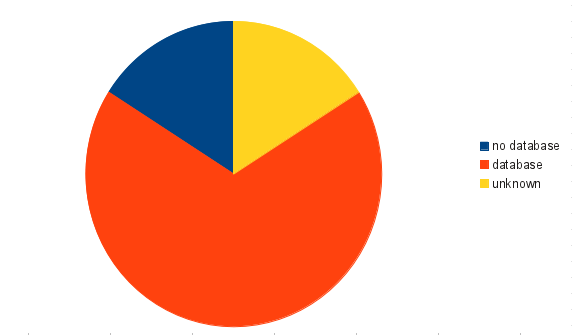
\includegraphics[width=0.8\textwidth] {Chart_database.png}
 }
 \subfigure[Software use of GIS;]{
   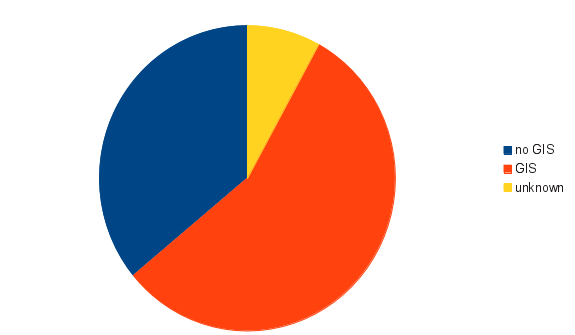
\includegraphics[width=0.8\textwidth] {Chart_gis.png}
 }
\caption[Aggregated analysis of the use of specific software components in the reviewed fisheries management systems;]
{Aggregated analysis of the use of specific software components in the reviewed fisheries management systems;}
\label{analysis1}
\end{figure}

The same conclusion can be drawn about GIS (see Figure~\ref{analysis1}b). The majority of systems uses a GIS component, or has a direct connection with GIS. However, the number of systems without GIS is close to the number of systems with GIS. 

\begin{figure}[ht]
\centering
\subfigure[Need of internet connection, in order to run the software;]{
   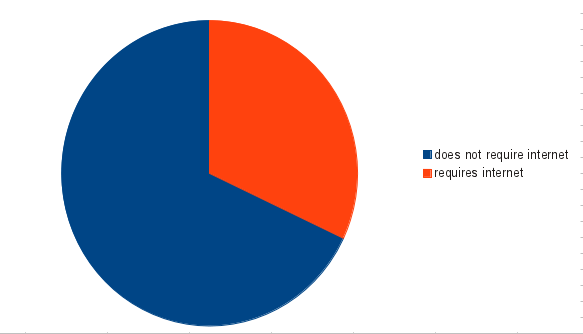
\includegraphics[width=0.8\textwidth] {Chart_internet.png}
 }
 \subfigure[Need for expert knowledge, in order to use the software]{
   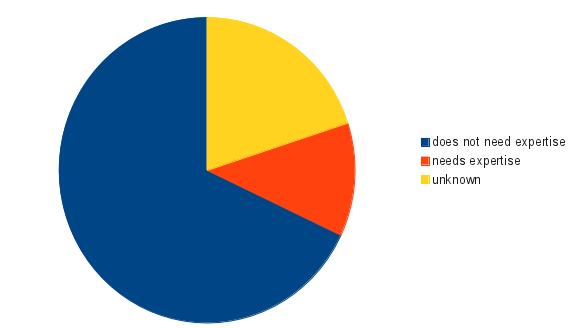
\includegraphics[width=0.8\textwidth] {Chart_expert.png}
 }
\caption[Aggregated analysis of specific characteristics the reviewed fisheries management systems;]
{Aggregated analysis of specific characteristics the reviewed fisheries management systems;}
\label{analysis2}
\end{figure}

As we can see in see figure~\ref{analysis2}a, the vast majority of the reviewed systems does not require an internet connection, in order to work. Also because some of the systems, are low in technology and make little (or no) use of the computer. However, it is important to note, that in modern systems there is an increase use of the server-client architecture, where they centralize the information (database, maps), and serve it through "thin" clients (normally web browsers). The use of web-mapping services such as WMS, triggered a "boom" in the adoption of this kind of model. It is important to note, that although the big advantage of this model is its distributed use, it may also possible to setup it locally on a LAN, or even on a single computer,

Most of the reviewed systems, whether they use software or not, do not present any information about the type of license in place (if any). This can be a consequence of the fact that most of the systems are not distributed, since they are nowhere available for download.

Moreover, most systems do not require a high knowledge of GIS, databases, statistics, etc, in order to be used (see figure~\ref{analysis2}b). This is either because: costum made solutions were implemented ("tailor-made" software), or widely-known software is used (like for instance MS Access). However, in some cases, specific tools are used that require a bit more literacy (for instance R); in this cases there is a trade-off, since there is something to gain in terms of potentialities of the software - it allows to perform more complex tasks - but it is also narrowed the number of possible adopters. 

  \begin{figure}[!ht]%[htbp]
    \begin{center} 
	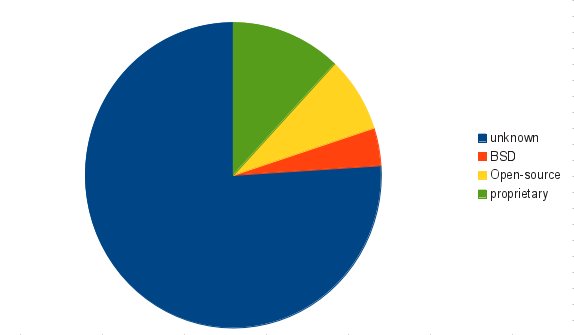
\includegraphics[width=\textwidth ]{Chart_license.png}
      \caption[Software licenses;] {Software licenses;}
      \label{licensing} % so that one can \ref it elsewhere	
    \end{center} 
  \end{figure}

As we can see in figure~\ref{licensing}, most of the reviewed systems, whether they use software or not, do not present any information about the type of license in place (if any). This may be a consequence of the fact that they are not widely distributed (?).

From the systems that specify licenses, there is the same amount of proprietary and open-source type licenses, which clearly indicates the co-existence of the two segments on the market. Looking at the timeline, there has been an increased adoption of "free and open-source-type" licences, and the expression of interest in adopting these licenses in systems that still rely on proprietary components. This is a very positive trend with great social impacts, specially regarding the adoption of these systems in developing countries (see section~\ref{foss}).

%\clearpage
The table bellow presents the 25 reviewed systems.

\tablefirsthead{%
\hline
\multicolumn{1}{|c|}{\textbf{Name}} & \multicolumn{1}{c|}{\textbf{Institution}} & \multicolumn{1}{c|}{\textbf{Description}} & \multicolumn{1}{c|}{\textbf{Technical Specifications}} \\ \hline
}
\tablehead{%
\hline
\multicolumn{4}{|l|}{\small\sl continued from previous page}\\
\hline
\hline
\multicolumn{1}{|c|}{\textbf{Name}} & \multicolumn{1}{c|}{\textbf{Institution}} & \multicolumn{1}{c|}{\textbf{Description}} & \multicolumn{1}{c|}{\textbf{Technical Specifications}} \\ \hline
}
\tabletail{%
\hline
\multicolumn{4}{|r|}{\small\sl continued on next page}\\
\hline}
\tablelasttail{\hline}
\bottomcaption{Table-resume of the reviewed Fisheries Management Systems}

\begin{center}
\begin{supertabular}{ | p{0.2\textwidth} | p{0.2\textwidth} | p{0.2\textwidth} | p{0.2\textwidth} |}
Fishframe & ICES & Web- based data warehouse application. It is a platform for data compilation and tabulating, that allows: upload of information, data quality control, data integration and raising. & Modularized software architecture; server client architecture; browser independent; well specified format; \\ \hline
InterCatch & ICES & Web-based system for handling fish stock assessment data, focusing on documenting characteristics of the catches.  & Client-server architecture (runs on a browser); it uses ASP and SQL Server; \\ \hline
ICES Spatial Facility & ICES & Free interface for searching, viewing and downloading spatial data. & WMS service (Geoserver) and client (OpenLayers); it was developed in PHP, with an SQL Server database and makes use of the Geonetwork; \\ \hline
ICES EcoSystem Data & ICES & Spatial database; it uses the standards adopted by the user community for the dissemination, visualization and sharing of ICES raw spatial data. & WFS server and client(Geoserver, OpenLayers). MS SQL Server database. \\ \hline
FMS & Schooner Solutions & Software that allows fishermen to track and manage information on daily trap fishing activities; at the same time, it produces reports of catch and effort for the DO. & Stand-alone software that runs on Windows (98 to XP). \\ \hline
The Canadian Albacore Tuna Catch And Effort Relational Database & Oceanic Fisheries Program (SPC) & System that provides annual catch estimates for the Canadian albacore troll fishery based on sales slips, logbooks, and hail Information. & MS Access \\ \hline
TUFMAN & Oceanic Fisheries Program (SPC) & Database fishery management tool. It provides solutions for: data entry, data management, data quality control, administration, and reporting. & Server-client architecture; server in SQL Server and client in MS access (supports the free versions); the mapping is provided through a loose couple with Mapinfo; \\ \hline
Catch and Effort Query System (CES) & Oceanic Fisheries Program (SPC) & Menu-driven system, which allows member countries to extract summaries of operational logsheet data, aggregate public-domain catch and effort data, and annual catch estimates. & It uses Mapinfo for mapping. \\ \hline
Fishery Analyst Online version & MappaMondoGIS & Web-based application, to query fishery data, analyze and visualize temporal and spatial patterns of fishery dynamics. & It uses the Google and ArcGIS JavaScript APIs and the Dojo framework. \\ \hline
Fishery Analyst for ArcGIS 9.x and 10 & MappaMondoGIS & Software for the quantitative estimation and visualization of catch and effort and their variation in space and time, analysis of fishing vessel utilization, data quality control, and deriving information on the location of important economic and threatened species. & Developed in VBA (arcobjects), inside ESRI ArcGIS. The data is stored in DBF files. \\ \hline
FiRST & Collaborative effort across eight South and Southeast (World Fish Center) Asian Countries. & Data management system for scientific trawl survey data. It includes data summary and reporting functionality; outputs: catch, CPUE and biomass estimates. It includes visualization tools, an analytical routine to estimate biomass, and data import/export modules.  & Server-client architecture. Server in MS access/ SQL Server (Windows); client in a browser. \\ \hline
PESCART & Instituto Nacional de Investigação Pesqueira (IIP) & Database system for storing data from artisanal fisheries and effectuate some calculus and reports (catch, effort, CPUE). It includes an interface for data acquisition, analysis and reporting. & Developed in Microsoft Access 97 (Windows 98); the system is split in two databases: one contains the data and the other one the app (UI+processing); it uses some MS specific ActiveX (Microsoft FlexGrid Control 5.0) and Libraries (.e.g DAO) \\ \hline
Geocrust & University of Algarve (UALG) & System that uses Satellite data (VMS) to map effort and landings;  & Modular stand-alone application with embedded GIS. It was developed using: Visual Basic 6.0., ADODB and MapObjects 2.0 Pro. It uses a MS Access Database (2000). \\ \hline
Geocrust 2.0 (Geopescas) & University of Algarve (UALG) & Improvement of the Geocrust application, as a consequence of extending the methodology to the ground fish trawl flee, a larger period, and a larger geographical area. & The db was migrated to MySQL running on a Linux server (higher security). It were introduced Artificial Intelligence methods (automatic classification methods) for trawl detection, in addition to the manual procedures. \\ \hline
Geopescas Website & University of Algarve (UALG) & Website to disseminate geo-referenced information on fishing effort, landings, catches and catch rates, through fisheries researchers, fishery administration and fishing industry. It shows some of the maps generated by the Geocrust software and it offers dynamic mapping, using Geotools. & It uses the Geoserver mapping component, costumised through JAVA programming. \\ \hline
COST & Project financed by the European Commission under the call FISH/2006/15 – lot 2 & Open Source Tool for raising and estimating properties of statistical estimates derived from the Data Collection Regulation. & set of R libraries, with the following functionality: import and handle fisheries data, explore the data , estimate the parameters and related precision and do simulation. It relies on data in a well specified forma.t \\ \hline
Catch Assessment Survey and Statistical frame survey of the artisanal fisheries of Kontagora Reservoir & ? & Catch Assessment Survey and Statistical frame survey, that aims to sustain the formulating of management plan and policies for the Kontagora reservoir. & Count and weighting of the fish. \\ \hline
Artisanal Fisheries Data Collection And Management In Tanzania & UNU Fisheries Training Program Fisheries Division - Statistical Unit  & Simple sampling procedure, community based data collection model and specifying of types of data to be collected. This system also includes analysis methods and a "tax motivation" strategy. & MS excel, MS Access Database. \\ \hline
IFMP & Lake Victoria Fisheries Organization (LVFO)  & Catch Assessment Surveys, two-stage stratified sampling design and estimation of CAS-based Indicators. & data forms (paper), MS Excel. \\ \hline
Barahona Data Collection System & Barahona Data Col PROPESCAR-SUR project & National Data Collection System & it relies on paper records and the calculations are done" by hand". \\ \hline
Samaná Fisheries Development Project (CEDEP) & Japan? & Logbook recording system, for a small number of vessels. & ? \\ \hline
FISBOAT & IFREMER & Fisheries Independent Survey-Based Operational Assessment Tools. The tools tackle the major issue of unreliable fish stock assessment, through the use of new methods based exclusively on research vessel survey data. & R, FLR simulation framework (R based) \\ \hline
Probability-based survey techniques in Mozambique & Instituto Nacional de Investigação Pesqueira (IIP) & Probability-based survey techniques for monitoring catch and effort in the coastal small-scale fisheries. & onsite survey, database (?) \\ \hline
Programme for refining estimates of local fishery production in Western Samoa & Peace Corps Marine Biologist Fisheries Division, Western Samoa & A programme for refining estimates of local fishery production, that consists in data collection(interviews) and data analysis; & It uses written down interviews to collect data and a hand-held programmable calculator for analysis; as a database, it is used DBASE III. \\ \hline
Electronic Fish Catch Logbook Project (EFCL) & Northwest Fisheries Centre (NWFSC) & Ship-based software and shore-based web application to collect and report logbook, catch "(fish tickets"), biological sample and observer data. There is also a report system, a central database and web based app to upload data. & Client server architecture, Oracle database, Arcinfo GIS; \\ \hline
\end{supertabular}
\end{center}
%\label{}
%\end{table}

In the following table, the reviewed systems are organized according to their technical characteristics:
\begin{itemize}
\item {\it internet}: indicates if the software needs an internet connection to work (binary value);
\item {\it GIS}: indicates if the software uses GIS (binary value);
\item {\it database}: indicate if the software uses a database (binary value);
\item {\it license}: indicates the type of license;
\item {\it portability}: comments about the cross-platform ability;
\item {\it expertise}: indicates if there is the need of expert knowledge to run the system (binary value);
\item {\it released}: indicates if the system is released and already in use; 
\end{itemize}

\tablefirsthead{%
\hline
\multicolumn{1}{|c|}{\textbf{Name}} & \multicolumn{1}{c|}{\textbf{internet}} & \multicolumn{1}{c|}{\textbf{GIS}} & \multicolumn{1}{c|}{\textbf{license}} & \multicolumn{1}{c|}{\textbf{database}} & \multicolumn{1}{c|}{\textbf{portability}} & \multicolumn{1}{c|}{\textbf{expertise}} & \multicolumn{1}{c|}{\textbf{released}} \\ \hline
}
\tablehead{%
\hline
\multicolumn{8}{|l|}{\small\sl continued from previous page}\\
\hline
\hline
\multicolumn{1}{|c|}{\textbf{Name}} & \multicolumn{1}{c|}{\textbf{internet}} & \multicolumn{1}{c|}{\textbf{GIS}} & \multicolumn{1}{c|}{\textbf{license}} & \multicolumn{1}{c|}{\textbf{database}} & \multicolumn{1}{c|}{\textbf{portability}} & \multicolumn{1}{c|}{\textbf{expertise}} & \multicolumn{1}{c|}{\textbf{released}} \\ \hline
}
\tabletail{%
\hline
\multicolumn{8}{|r|}{\small\sl continued on next page}\\
\hline}
\tablelasttail{\hline}
\bottomcaption{Reviewed Fisheries Management Systems, according to their characteristics}

\begin{center}
\begin{supertabular}{ | p{0.1\textwidth} | p{0.05\textwidth} | p{0.05\textwidth} | p{0.05\textwidth} | p{0.05\textwidth} | p{0.2\textwidth} | p{0.05\textwidth} | p{0.05\textwidth} |}
Fishframe & 1 & 1 & BSD & 1 & Since the clients are browser based, they are cross platform; the server has to run on Windows, since it uses Microsoft specific active technologies (ASP) & 0 & yes \\ \hline
InterCatch & 1 & \multicolumn{1}{l|}{?} & ? & 1 & Since the clients are browser based, they are cross platform; the server has to run on Windows, since it uses Microsoft specific active technologies (ASP) & \multicolumn{1}{l|}{?} & ? \\ \hline
ICES Spatial Facility & 1 & 1 & ? & 1 & Server and client are cross-platform. & 0 & yes \\ \hline
ICES EcoSystem Data & 1 & 1 & ? & 1 & Server and client are cross-platform. Database is Windows specific. & 0 & yes \\ \hline
FMS & 0 & \multicolumn{1}{l|}{?} & proprietary & \multicolumn{1}{l|}{?} & Windows only (98 to XP) & \multicolumn{1}{l|}{?} & under final modifications \\ \hline
The Canadian Albacore Tuna Catch And Effort Relational Database & 0 & 1 & ? & 1 & Windows only & 0 & yes \\ \hline
TUFMAN & 0 & 1 & ? & 1 & Windows only & \multicolumn{1}{l|}{?} & yes \\ \hline
Catch and Effort Query System (CES) & 0 & 1 & ? & 1 & Windows only & 0 & yes \\ \hline
Fishery Analyst Online version & 1 & 1 & proprietary & \multicolumn{1}{l|}{?} & The client is free and cross platform (runs on a browser) & 0 & yes \\ \hline
Fishery Analyst for ArcGIS 9.x and 10 & 0 & 1 & proprietary & 1 & Windows only & 1 & yes \\ \hline
FiRST & 1 & 1 & ? & 1 & Since the client runs on a browser, it is platform independent. Server runs on Windows. & 0 & yes \\ \hline
PESCART & 0 & 0 & ? & 1 & Windows only & 0 & yes \\ \hline
Geocrust & 0 & 1 & ? & 1 & Windows only & 0 & yes \\ \hline
Geocrust 2.0 (Geopescas) & 0 & 1 & ? & 1 & The application runs on Windows, but the database can now run on Windows or Linux. & 0 & yes \\ \hline
Geopescas Website & 1 & 1 & ? & 1 & ? & 0 & demo version only \\ \hline
COST & 0 & 1 & Open-Source & 1 & since it relies in R, it is cross-platform. & 1 & yes \\ \hline
Catch Assessment Survey and Statistical frame survey of the artisanal fisheries of Kontagora Reservoir & 0 & 0 & ? & \multicolumn{1}{l|}{?} & ? & 0 & yes \\ \hline
Artisanal Fisheries Data Collection And Management In Tanzania & 0 & 0 & ? & 1 & Windows only & 0 & yes \\ \hline
IFMP & 0 & 0 & ? & 0 & Windows only & 0 & yes \\ \hline
Barahona Data Collection System & 0 & 0 & ? & 0 & n/a & 0 & yes \\ \hline
Samaná Fisheries Development Project (CEDEP) & 0 & 0 & ? & 0 & ? & \multicolumn{1}{l|}{?} & yes \\ \hline
FISBOAT & 0 & 0 & Open-source & 0 & multi-platform & 1 & yes \\ \hline
Probability-based survey techniques in Mozambique & 0 & 0 & ? & \multicolumn{1}{l|}{?} & ? & \multicolumn{1}{l|}{?} & yes \\ \hline
Programme for refining estimates of local fishery production in Western Samoa & 0 & 0 & ? & 1 & Windows only (DOS) & 0 & yes \\ \hline
Electronic Fish Catch Logbook Project (EFCL) & 1 & 1 & ? & 1 & Some components run on a browser, so they may be cross-platform, but the database and GIS are Windows only. & 0 &  \\ \hline
\end{supertabular}
\end{center}

The next table, goes a bit more in depth, and it analyses some of the advantages and disadvantages of each system. 

\tablefirsthead{%
\hline
\multicolumn{1}{|c|}{\textbf{Name}} & \multicolumn{1}{c|}{\textbf{Advantages}} & \multicolumn{1}{c|}{\textbf{Disadvantages}} \\ \hline
}
\tablehead{%
\hline
\multicolumn{3}{|l|}{\small\sl continued from previous page}\\
\hline
\hline
\multicolumn{1}{|c|}{\textbf{Name}} & \multicolumn{1}{c|}{\textbf{Advantages}} & \multicolumn{1}{c|}{\textbf{Disadvantages}} \\ \hline
}
\tabletail{%
\hline
\multicolumn{3}{|r|}{\small\sl continued on next page}\\
\hline}
\tablelasttail{\hline}
\bottomcaption{Advantages and disadvantages of each system}

\begin{center}
\begin{supertabular}{ | p{0.3\textwidth} | p{0.3\textwidth} | p{0.3\textwidth} |}
Fishframe & - data ownership of the recipients; - deals with incomplete data; - cross platform); - enforces confidentiality; - involvement and engagement of stakeholders; - bottom-up approach & - some components require Windows XP; - development is Windows based; - for complex tasks the browser solution is not efficient; \\ \hline
InterCatch & ? & It uses proprietary and platform-specific software \\ \hline
ICES Spatial Facility & - cross platform (browser based); - adopts OGC standards; - friendly UI; - uses Free and Open Source Software( FOSS); & There is no component of data acquiring in this system; it is assumed the raw data is validated. \\ \hline
ICES EcoSystem Data & - cross platform (browser based); - adopts OGC standards; - friendly UI; - uses Free and Open Source Software( FOSS); & - some requests may be slow due to the quantity of data; - - it deals only with survey data; \\ \hline
FMS & It does not require a very powerful hardware to run. & - it runs only on windows; -it has a cost; \\ \hline
The Canadian Albacore Tuna Catch And Effort Relational Database & - it deals with unreported catch; - although it is a post-season analysis tool, in can be used as in-season analysis (based only on trip logs); & - the results may be biased due to the use of logbooks without saleslip data; - other sources of bias are the "public sales" and "take homes" that are not registered anywhere (they "escape" from logbook and sales slips);  \\ \hline
TUFMAN & - the website provides excellent documentation on how-to use the application; - flexible system, able to cater the needs of each country; - it allows to identify gaps in data; & - it uses proprietary components (Mapinfo, Microsoft Office Pro); - it does not feature data acquisition, and therefore it is dependent on the quality of input data; - it does not provide tools to fill the gaps in the data; - it is not found anywhere to download; \\ \hline
Catch and Effort Query System (CES) & - developed reporting facilities, with the use of graphs, tables and maps; & - it uses proprietary components (Mapinfo); - it is not found anywhere to download; \\ \hline
Fishery Analyst Online version & - lightweight and cross-platform application; & -it has a cost; \\ \hline
Fishery Analyst for ArcGIS 9.x and 10 & - it takes advantage of GIS to analyze geodata; - it provides a time series animation; - it provides data quality control routines; - it uses; transversal information (economical); - confidentiality is addressed; & - it has a cost, although a demo version is provided for free; - it requires ArcGIS 8.3. or 9 with Spatial Analyst (and it needs this specific versions to work); - iit requires some knowledge of ArcGIS to use; - it requires some detailed georeferenced data to start with (no estimation provided!) \\ \hline
FiRST & - client is cross platform; - no installation required for the client; - a regional database is “compiled” from the national databases; - outputs can be used for ecological modelling (very useful for management – devise or revise zonation schemes); & - the database is designed for scientific trawl surveys; - it requires installation of a webserver; - the exporter uses mostly proprietary formats (MS Office, Crystal reports, MS Access); \\ \hline
PESCART & - intuitive UI following the information flow; - it is a very complete system, since it covers: data acquisition, estimation and reporting. & - it targets artisanal fisheries only (the basic unit is fishing unit); - "bulky" setup with a lot of requirements; - the application does not have any access restrictions (no permission system implemented); - the limitations of MS Access "clash" with the design of the app (e.g. number of fields on a table does not allow the selection of a large number of species;) \\ \hline
Geocrust & - it combines positioning and landing data, from different sources (IGP, DGPA, logbooks); - extense use of GIS, not only for display but also for calculations (e.g.: buffers to define start and end of fishing trips); - it is generic enough, to be used with other fleets/geographic areas/species; & - it is based on proprietary technologies; - it relies on accurate positioning data (VMS); - it was not addressed a permission model for the UI (only superuser); \\ \hline
Geocrust 2.0 (Geopescas) & - the procedure of identification of trips was enhanced with AI; - DBMS was migrated to a free, multi-platform software; & - it is still based on proprietary technologies; - the AI procedure needs adequate "training", in order to produce good results; \\ \hline
Geopescas Website & - it provides an interface for querying maps; - it exports georeferenced maps, images and XML, that can be integrated in third-party apps.  & - it depends on technologies Ggeotools) that are heavy on the browser and require the installation of the Java plugin; - it was only released a demo version; \\ \hline
COST & - space dimension is included in the analysis; - uses well known technology; - promotes import and export of data; - open source and cross platform tool; - interfaces with Fishframe format; & - relies in good quality and well formatted data; - it requires expert knowledge; \\ \hline
Catch Assessment Survey and Statistical frame survey of the artisanal fisheries of Kontagora Reservoir & - it is a complete system, including data collection (survey) and statistical analysis of the results; - it comprehends both effort and catch; & Although the data is collected spatially, there is no indication that this component is taken in account in the sampling and analysis. \\ \hline
Artisanal Fisheries Data Collection And Management In Tanzania & - relatively inexpensive; - it does not need specialized staff to run and maintain it; - it contemplates the community participation; & There is no reference to GIS in the sampling procedure (although the sampling is on space), or in the estimation process. \\ \hline
IFMP & - it provides estimations of the catch over the years, which allows to detect trends, to detect need for further data and to evaluate management interventions. & - since data collection is through papper sheets, there is no data quality control on introduction; - there is no mention of a solution to store and manage the data over time (DB); - there is no use of GIS, although the PSU are spatial; \\ \hline
Barahona Data Collection System & - the economic variables are well catered; - it gathers relatively accurate catch and effort information based on trip interviews; The effort variables, in particular, seem well thought out and adequate for monitoring CPUE and estimating fishing mortality; - the system was sustained, even after withdraw of external funding; & - mortality and growth cannot be estimated with current data ; - there is the need for a new approach fro estimating discards; - the current sampling procedure does not follow a statistically rigorous method. - there is no database to store and manage data on a long term; - there is the need of training; - stock assessment is not contemplated in this system; \\ \hline
Samaná Fisheries Development Project (CEDEP) & - data collection is rigorous; & - the logbooks are not formally structured; - the data is not maintained in a database; \\ \hline
FISBOAT & - these tools provide robust and reliable scientific advice to fishery managers and policy-makers, including a management model driven by numerically defined harvesting rules; - it is provided an early-warning mechanism, giving policy-makers more time to respond pro-actively to evolving challenges. & - the methods are based exclusively on research vessel survey data; - it requires expert knowledge to be used (statistics and computation); \\ \hline
Probability-based survey techniques in Mozambique & - the probability sampling produces unbiased estimates of catch, effort, and other key parameters; - the precision in such estimates can be quantified; - it is cost-effective; - the underlying theory is well developed and documented; & - no mentioning of use of GIS; \\ \hline
Programme for refining estimates of local fishery production in Western Samoa & - cost-effective method of gathering basic information that provides clues to changes in the fishery as a whole; - it requires a small input of resources for the information obtained; & - the data quality of the survey is threatened by the hiring of causal workers, without adequate supervision; the same for data entry in the database; - outdated database technology; - there is the need to collect more data (from the villages) to estimate the catch; - there is the need to design more complete entry datasheets; \\ \hline
Electronic Fish Catch Logbook Project (EFCL) & - innovative effort to automate and standardize logbook data. - it implements permissions through roles; - it supports secure connections (data encryption) - the use of a software to input the raw data, allows a first validation layer that does not exist in traditional systems using papper sheets; - costumisable;  & - it is based in proprietary technologies; - it relies on internet access for data uploads and visualization; \\ \hline
\end{supertabular}
\end{center}

On section~\ref{objectives} we present a set of fishery management tools that aim to fill some of these "gaps" on existent systems, reusing some of its (good) ideas and adding new technologies that are "giving cards" on other fields (like fuzzy mapping, on section~\ref{output}, or artificial intelligence), keeping in mind the limitations faced by potential adopters (developing countries). Some of these ideas arised during the development of Medfisis-CAS~\cite{medfisis}, an (almost) full free and open-source system that brings together data from Logbook and Artisanal Fisheries in the same application/database; some of the concepts developed during this project such as abstractability of entities (see section~{reuse}) and configurability of components can be very useful in all aspects of fishery data management systems.\\
Figure~\ref{challenges} shows some of the challenges that can be addressed by a set of fisheries management tools. We propose a loose couple architecture, where we maximize the use of existing tools: to cut development time, to benefit from their value and also to involve a community of users that can take advantage of their expertise in specialized tools (like for instance R, or QGIS) to push the system further. The modularization of the system also means that we can distribute tasks, and to a certain extent develop them independently without compromising the rest of the system.\\

%open source
%creation of a community /AGILE model for development
%improvement of the manuals
%success stories in other areas 

  \begin{figure}[!ht]%[htbp]
    \begin{center} 
	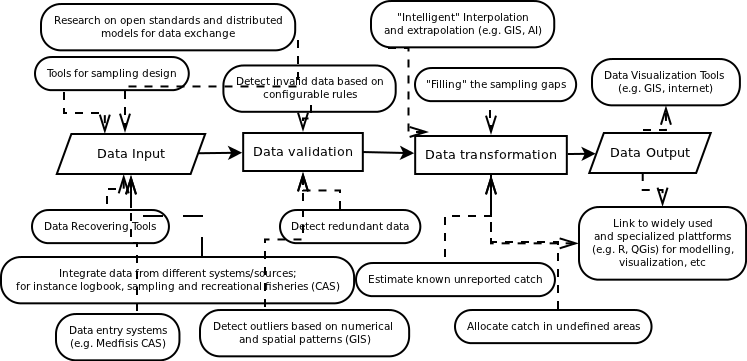
\includegraphics[width=\textwidth ]{challenges_cas}
      \caption[Some Interesting Challenges on Fishery Management Systems;]{Some Interesting Challenges on Fishery Management Systems;}
      \label{challenges} % so that one can \ref it elsewhere	
    \end{center} 
  \end{figure}

\clearpage

\section{Project Objectives}\label{objectives}
The design of a software system for fishery management, as described in section~\ref{background} (figure~\ref{challenges}), should contemplate four stages:
\textbf{input, validation, transformation and output}. The main target for each of these stages is the data about fisheries, in its raw or transformed state (catch, efforts), but it can also be other (complementary) data (meteorological, oceanographical, socio-economic, etc). In the following subsections we identify a serious of tasks that are \textit{on-demand}, and could result in very useful tools for fisheries scientists and managers. %They are not limitative, and in
In our modular design they can be seen as a first approach rather than a complete description of the system.\\

\subsection{Data Input}\label{input}
The data input component contemplates the collection of information for the system, either by creating this information "from scratch" or by importing it from different supports/formats.

\begin{itemize}
  \item \textbf{Tools for Sampling Design}: Before even introducing information in the system, it is often necessary to collect this information; the design of an unbiased sampling scheme, that minimizes the costs and maximizes the quality of the results is an important and often overlooked task; overlooked, because often the designer does not possess the tools to make it an easy and efficient process. There are many advantages of using a spatial framework (GIS) on this particular problem, and suggestions can guide the sampler to informed and wise decisions.
  \item \textbf{Research on Open Standards and Distributed Models for Data Exchange:} The problem of exchanging data between different instances of the system is a pertinent and frequent one. JSON~\cite{json} %and SQLite~\cite{sqlite} are%
is an open and well-known standard that constitutes a "light" alternative to XML. Also, the design and implementation of a server-client model, where we leave the "heavy processing load" to the server and create "light" data acquiring clients (for instance running on mobile phones and tablet PCs) can simplify the task of data integration, as we only update restricted parts of the system. On section~\ref{nosql} we discuss the possibility of implementing a distributed system, using a non-relational model.
  \item \textbf{Data Recovering Tools:} There is a large quantity of historical data that is lost in terms of its value, just because it is not in an usable format. Data series take many years to assemble: not only it costs a lot of money to generate new data, but it is not actually possible to recreate past information; thus when this information is lost, it is lost forever. It could be a very rewarding task to at least try to compile this information, that may not be usable for different reasons; hard disks that have bad sectors, obscure data formats whose specification was lost, data in non digital support and nearly illegible: these are all problems eligible for "data archaeology", that can make use of "sophisticated" software techniques such as: writing recognition, deyncription algorithms and hard-disk recover tools.
  \item \textbf{Integrate data from different systems/sources:} The integration of different types of information provides a rich basis for the analysis and transformation of information; this includes having data from different sources such as oceanographical, meteorological, sociological, etc; apart from implementing a system that is able to import different formats (satellite images, excel spreadsheets, vector maps, etc) it is also relevant to design a system that can deal with the nature of this variability - for instance recreational fisheries data, logbooks and sales slips can be integrated with a unified and generic design and provide a richer basis for fisheries statistical analysis (see~\cite{medfisis}).
  \item \textbf{Data Entry User Interfaces:} Database clients are a \textit{milestone} in fisheries applications and common examples of this are digital logbooks and fleet register software's (see~\cite{medfisis}). They reproduce the behavior of paper sheets for data collection, with all the advantages of data checking, and "feed" directly the database; if well designed and data operators are trained, they are also quicker and more friendly to use than the replaced papper sheets. There is still a room for improvement on this UIs, for instance enabling multiple choices or configurable validation rules~\footnote{As an example, some of this features were already implemented in CAS Medfisis~\cite{medfisis}}.
\end{itemize}

  \begin{figure}[!ht]%[htbp]
    \begin{center} 
	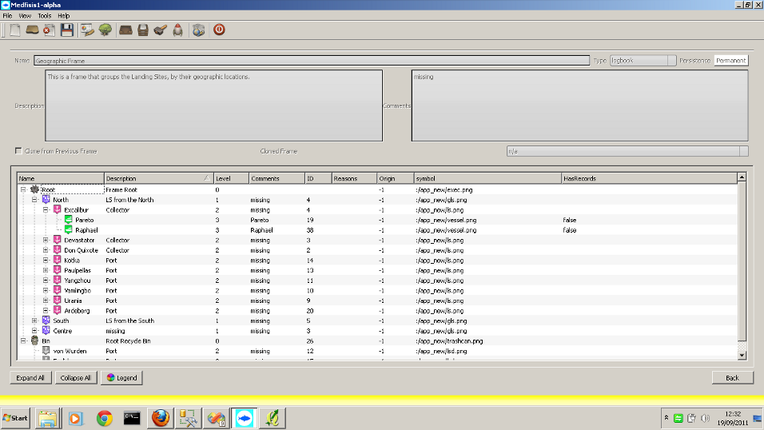
\includegraphics[width=\textwidth ]{geographic_frame}
      \caption[This \textit{tree-like} widget is a tool developed in Medfisis~\ref{medfisis} to assist in the design of a sampling frame; the user can drag and drop elements from one group to another, which can be an interesting feature for designing sampling schemes;] {This \textit{tree-like} widget is a tool developed in Medfisis~\cite{medfisis} to assist in the design of a sampling frame; the user can drag and drop elements from one group to another, which can be an interesting feature for designing sampling schemes;}
      %\label{challenges} % so that one can \ref it elsewhere	
    \end{center} 
  \end{figure}


  \begin{figure}[!ht]%[htbp]
    \begin{center} 
	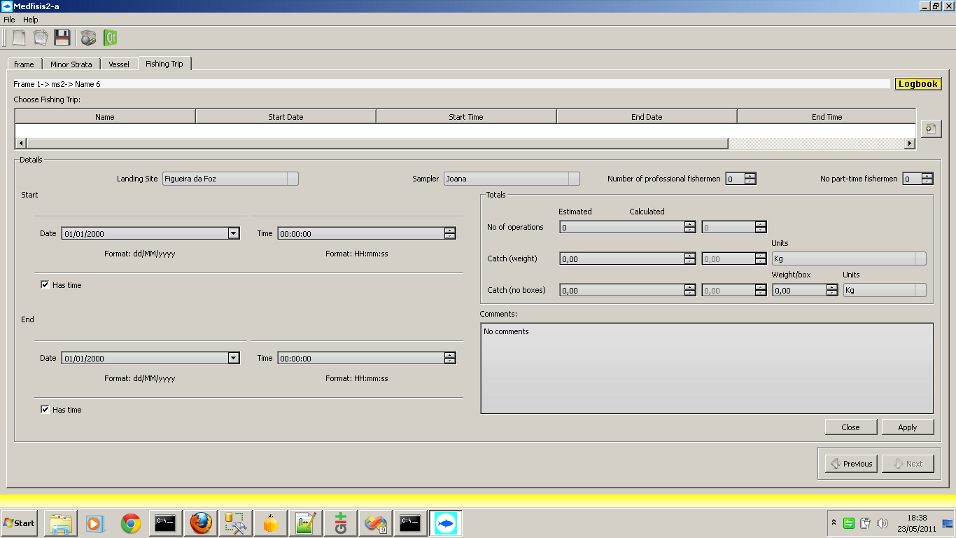
\includegraphics[width=\textwidth ]{fishing_trip_small}
      \caption[Screenshot of a data entry form for fishing tip data, on CAS Medfisis~\cite{medfisis}; on this system, forms were designed to accommodate at the same time logbook and artisanal fisheries data;] {Screenshot of a data entry form for fishing tip data, on CAS Medfisis~\cite{medfisis}; on this system, forms were designed to accommodate at the same time logbook and artisanal fisheries data;}
      %\label{challenges} % so that one can \ref it elsewhere	
    \end{center} 
  \end{figure}

\subsection{Data Validation}\label{validation}
Since the data entering the system may arrive from sources other than its data generator interfaces\footnote{The data entry interfaces should have already their own validation routines removing, at least partially, the need for this step.}, it is important to control the quality and validity of information we are inputing; this step is fundamental for all the following ones, since "bad quality" data will compromise the entire system ("garbage in, garbage out").\\
The Fishframe application~\cite{fishframe}, developed by the Danish Institute for Fisheries Research, presents an interesting and complete multi-step validation layer; on a first stage it is performed a basic check, looking at the structure of the data, ranges of values and duplicate values; on a second stage, a more complex check searches for the correctness of the dependency between fields; finally, the last check (which is not compulsory) performs a global analysis, looking at the general patterns in order to identify outliers. Apart from this, it also allows some customizable checks to be introduced by the user, that can be performed automatically. This flexibility and completeness of the validity step, inspired us to identify the following tasks in the data validation component of this system:

\begin{itemize}
  \item \textbf{Detection of redundant data}: The detection (and consequent removal) of duplicate records is an important task, in order to have a "clean" database. It is not complicate to identify automatically records that are \textbf{exactly} identical, but the problems arise when we have for instance spelling mistakes, and records that are \textit{almost} the same, but not exactly the same. As this situations are dubious, and may correspond or not to duplicate data, they require user supervision to confirm it; however, there is no reason why they can not be identified and presented to the operator has "possible duplicates"; for this task, it is very useful to use data mining techniques such as a fuzzy approach to language~\cite{fuzzy}.

  \item \textbf{Detection of invalid data based on configurable rules}: Generic rules can be applied to check for the correctness of the data types, correctness of keys, etc, directly based on the database schema. However, some rules such as the format of strings, ranges of values, may change from system to system  (for instance according to the geographic location) and the option to create them should be left to the user. To avoid "hard-coding" of rules, which would require a programmer's intervention and consequently difficult the process of exploratory analysis, we propose an interface for user configurable rules. This interface can be similar to a query builder such as the one represented in~\ref{builder}, which may be familiar to some users.

  \item \textbf{Detection of Outliers}: Outliers may arise due to "careless" data acquiring, instrument malfunction, wrong data processing routines, or any other reasons~\cite{outliers}; generic methods based on tabular data (for instance using a principal component analysis) can be used to perform this task, but there is also room for other techniques such as data mining, or GIS; for data with a spatial distribution (which is often the case in fisheries) GIS can provide a very valuable tool for capturing the general spatial pattern and consequently the values that fall outside this pattern (outliers)(see figure~\ref{dem}).
  After detecting and removing outliers values, we are left with the problem of imputation of "missing values" to replace the removed information (see section~\ref{transformation})

\end{itemize}

  \begin{figure}[!ht]%[htbp]
    \begin{center} 
	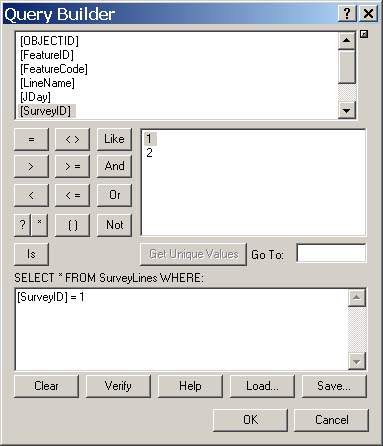
\includegraphics[width=0.5\textwidth ]{builder.jpg}
      \caption[Query builder from ArcGIS;]
{Query builder from ArcGIS; source:~\url{http://woodshole.er.usgs.gov/pubs/of2006-1381/html/fig19.html};}
      \label{builder} % so that one can \ref it elsewhere	
    \end{center} 
  \end{figure}

  \begin{figure}[!ht]%[htbp]
    \begin{center} 
	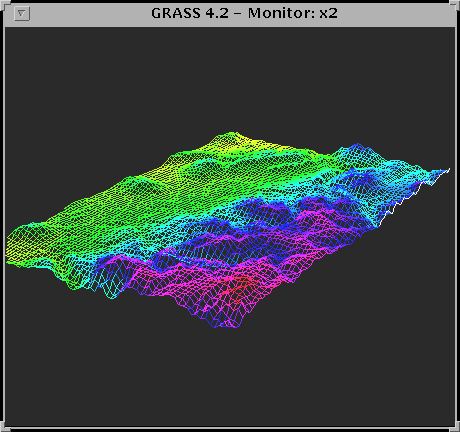
\includegraphics[width=0.8\textwidth ]{dem.png}
      \caption[A Digital Elevation Model (DEM) like the one above, can be used to generate a surface of values in order to detect outliers;]
{A Digital Elevation Model (DEM) like the one above, can be used to generate a surface of values in order to detect outliers; source:~\url{http://www.grass-kr.org/research/demo1/index.html};}
      \label{dem} % so that one can \ref it elsewhere	
    \end{center} 
  \end{figure}


\subsection{Data Transformation}\label{transformation}
Data transformation consists in using the information in the system and apply transformations to it, in order to generate new information. These transformations may be used to estimate values extending the scope of the dataset, or to generate indicators that characterize the dataset, like for instance the CPUE, or both. In this system we suggest facilitating the export of data and leave (some) more complex data analysis to specialized software such as R (figure~\ref{lengths}) or QGIS (figure~\ref{layers}).

  \begin{figure}[!ht]%[htbp]
    \begin{center} 
	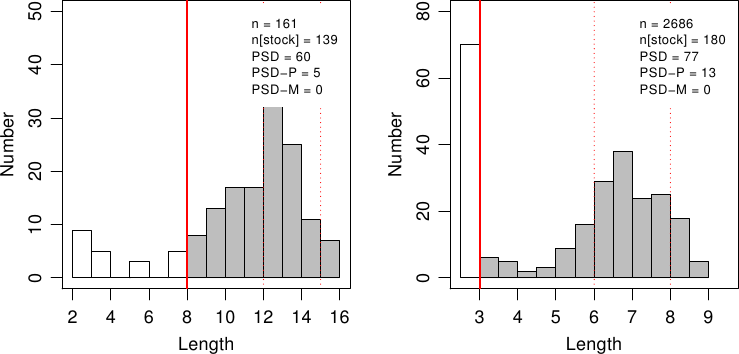
\includegraphics[width=\textwidth]{lengths}
      \caption[This analysis of the size structure was created using the R package;]
{This analysis of the size structure was created using the R package; source:~\url{http://www.ncfaculty.net/dogle/fishR/index.html};}
      \label{lengths} % so that one can \ref it elsewhere	
    \end{center} 
  \end{figure}

  \begin{figure}[!ht]%[htbp]
    \begin{center} 
	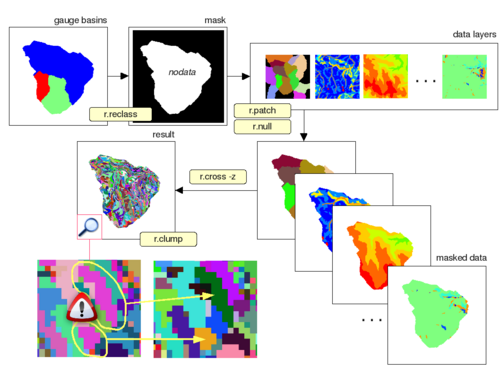
\includegraphics[width=\textwidth]{layers}
      \caption[QGIS (in this example using the grass functionality) can be used to overlay different types of information;]
{QGIS (in this example using the grass functionality) can be used to overlay different types of information; source:~\url{http://geoinformatics.fsv.cvut.cz/gwiki/Deriving_Hydrological_Response_Units_\%28HRUs\%29_using_a_Web_Processing_Service_implementation_based_on_GRASS_GIS};}
      \label{layers} % so that one can \ref it elsewhere	
    \end{center} 
  \end{figure}

Bellow are examples of some specific (and common) problems with catch data, for which we propose to develop some solutions in the system.% One is that we are missing data from our sampling universe (for instance it is an outlier or simply it was not sampled); the other is the data exists, but it is incomplete since the 

\begin{itemize}
  \item \textbf{Imputation of missing data}: Under-sampled or non sampled strata lead to an unknown bias, a problem that should be reduced with a good sampling design~\cite{ices}. For the situations where we have to deal with missing values, it is possible to inmputate them, having in mind that also the method used for this operation can introduce some bias in the system. According to ICES~\cite{ices} automatic methods should be avoid, in favor of expert knowledge, but they can be aided by spatial modelling techniques having in mind that to be use with success the spatial distribution should remain stable over time; this is a cue for developing GIS based models, that can provide the expert with a good basis for informed choices.

  \item \textbf{Allocate Catch in undefined areas}: On the Canadian Albacore Tuna Catch and Effort Relational Database~\cite{tuna} it is presented the problem of having sales or logbook catch data, whose geographic area is undefined. Instead of discarding these values from the calculations of catch by area, the authors found ways to distribute the catch and effort, following the overall geographic pattern of fleet; they allocate these values in proportion with the total catch and vessel distribution and for this purpose GIS can be very useful, for instance to produce a grid, or a contour map (see figure~\ref{kernel}) with frequencies.

  \item \textbf{Estimate known unreported catch}: Another delicate problem arises from the incomplete vessel count. If there is an unreported effort than it will probably be reflected in an unreported catch. For the cases where it is known that an unreported effort exists, the authors of the the Canadian Albacore Tuna Catch and Effort Relational Database~\cite{tuna} suggest to extrapolate the total catch estimates based, on estimated number of unreported vessels. According to~\cite{morocco}, unreported catch can be as significant as 50\% of the total catch and therefore it is important to find suitable methods to approach this problem, like for instance the Monte Carlo Simulation (see figure~\ref{montecarlo}).

\end{itemize}

  \begin{figure}[!ht]%[htbp]
    \begin{center} 
	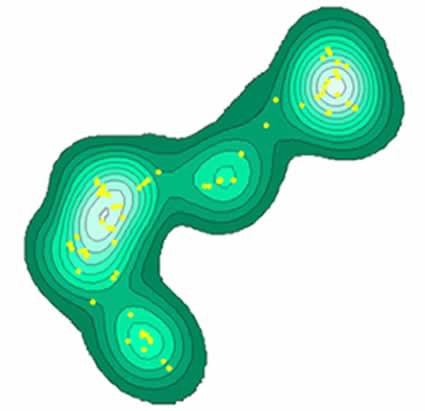
\includegraphics[width=0.5\textwidth]{kernel}
      \caption[The Kernel Home Range Method is a probability measurement that outputs contours, based on punctual observations;]
{The Kernel Home Range Method is a probability measurement that outputs contours, based on punctual observations; source:~\url{http://www.bio.davidson.edu/people/midorcas/GISclass/GISprojects/grayson/GISMethods.htm};}
      \label{kernel} % so that one can \ref it elsewhere	
    \end{center} 
  \end{figure}

  \begin{figure}[!ht]%[htbp]
    \begin{center} 
	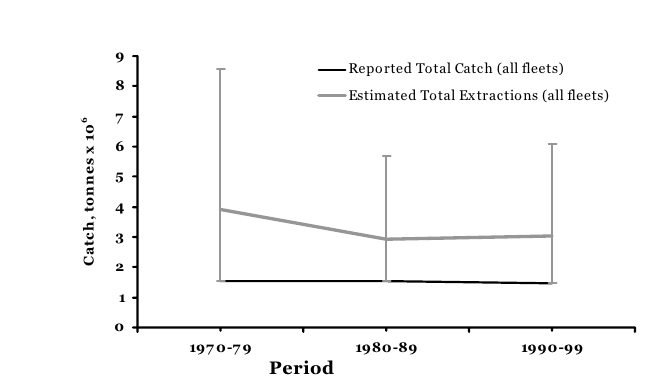
\includegraphics[width=\textwidth]{montecarlo}
      \caption[In this example, Monte Carlo Simulation was used to elaborate estimates of total extractions of all species from Moroccan waters; in the image we see the comparison with the total reported catch;]
{In this example~\cite{morocco}, Monte Carlo Simulation was used to elaborate estimates of total extractions of all species from Moroccan waters; in the image we see the comparison with the total reported catch;}
      \label{montecarlo} % so that one can \ref it elsewhere	
    \end{center} 
  \end{figure}

%Apart from this, interpolation/extrapolation algorithms could be developed to deal with different types of information (effort, catch, climatological data, etc).

\subsection{Data Output}\label{output}
Data output, of raw or transformed information, is a component where it is possible (and desirable) to facilitate the link with other platforms by using "friendly" and well-known formats. This could include formats for tabular data (for excel, R, etc), but also formats for spatial data (shapefiles, GeoJSON,etc).\\
GIS provide some very-rich and expressive visualization tools with a great potential for fisheries data, that we will discuss summarily in the next few paragraphs.\\
Web mapping is the process of designing, implementing, generating and delivering maps on the World Wide Web~\footnote{\url{http://en.wikipedia.org/wiki/Web_mapping}}. Compared to "traditional" maps, maps on the Internet have many other advantages such as "live updating", and link with many other sources of information; they provide the same interactivity as a GIS software, with the advantage of not requiring a specific software client, since they can run on an Internet browser. Web maps are normally incorporated in portals together with other types of information, the case of ICES Ecosystem Data~\cite{ices2} (see figure~\ref{webmap}), but they can also be embedded in a software application (see figure~\ref{marble}).

  \begin{figure}[!ht]%[htbp]
    \begin{center} 
	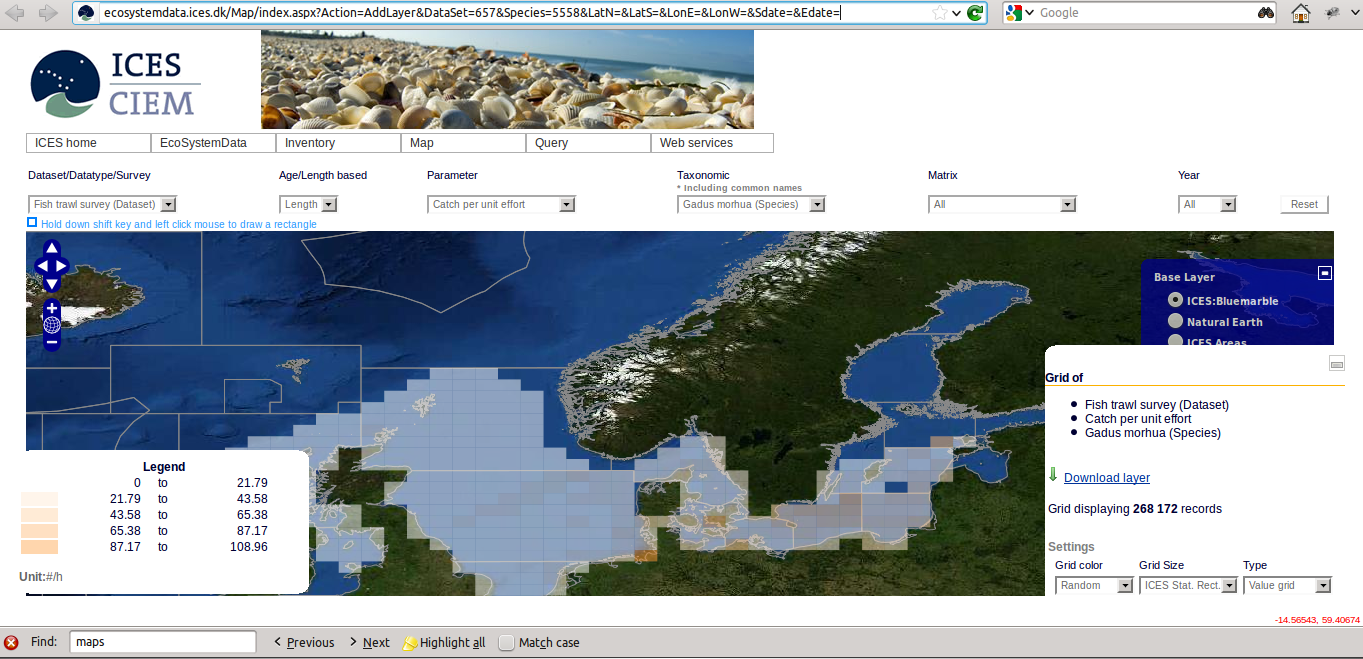
\includegraphics[width=\textwidth]{webmap}
      \caption[Web map of a ICES fish trawl Survey dataset, overlaying a grid of CPUE on top of a layer of Marble (Nasa Worldwind);]
{Web map of a ICES fish trawl Survey dataset, overlaying a grid of CPUE on top of a layer of Marble (Nasa Worldwind)~\cite{ices2};}
      \label{webmap} % so that one can \ref it elsewhere	
    \end{center} 
  \end{figure}

  \begin{figure}[!ht]%[htbp]
    \begin{center} 
	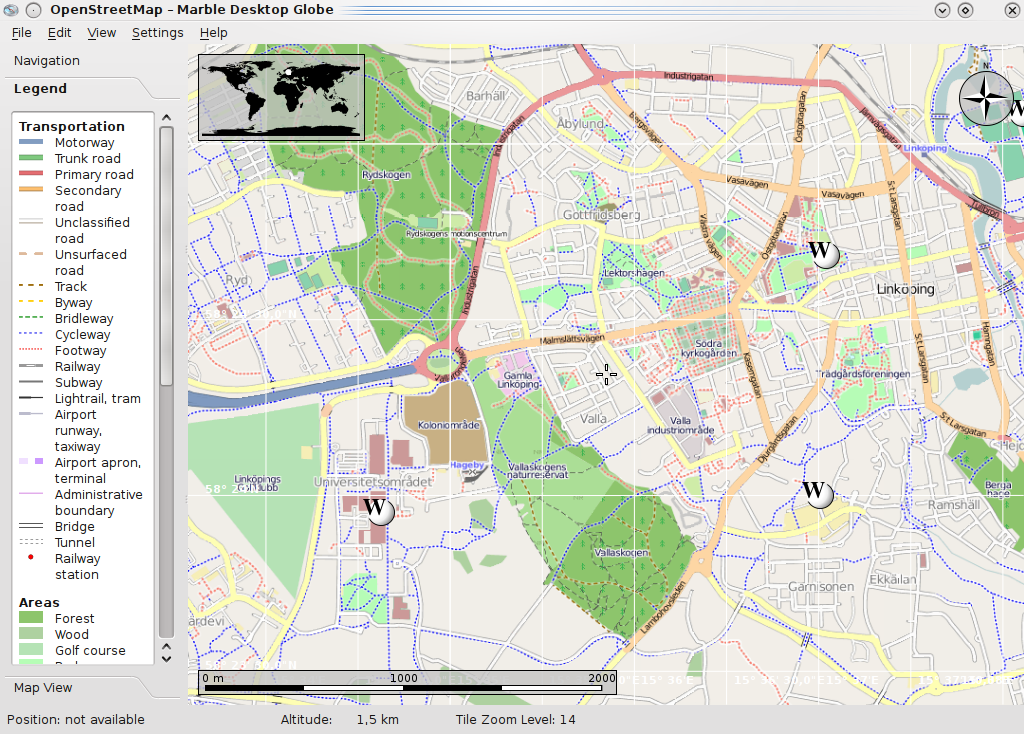
\includegraphics[width=\textwidth]{marble}
      \caption[Marble is a free and open source application that displays webmaps, along with other types of maps in a C++ application;]
{Marble~\footnote{\url{http://edu.kde.org/marble/}} is a free and open source application that displays webmaps, along with other types of maps in a C++ application; source:~\url{http://edu.kde.org/marble/screenshots/generic/marble-linkoeping.png};}
      \label{marble} % so that one can \ref it elsewhere	
    \end{center} 
  \end{figure}

Continuous maps showing densities, can be created using grids or contours or other methods such as TINs. Grids (such as the one on figure~\ref{webmap}) are very common to represent distributions of fishing effort or catches; On the Geocrust project (see~\cite{geocrust}), the generation of grids with different sizes allowed the user to have a more generalized or more detailed perception of the fishing effort, which calls its attention to different properties (see figure~\ref{grids}).

\begin{figure}[ht]
\centering
\subfigure[Density map of fishing effort, using a large grid;]{
   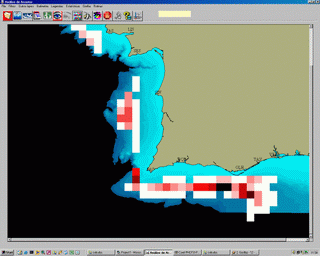
\includegraphics[width=0.8\textwidth] {densidades99_5x5}
 }
 \subfigure[Density map of fishing effort, using a small grid;]{
   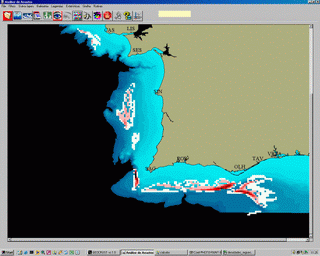
\includegraphics[width=0.8\textwidth] {densidades99a.png}
 }
\caption[Fishing effort maps generated by GeoCrust 2.0. To produce these maps the user can choose one or more vessels for a given period of time quarter, semester, and year); VMS data from valid fishing trips trawl hauls. Density grid size set by the user (minimum 0.06 x 0.06 nm);]
{Fishing effort maps generated by GeoCrust 2.0. To produce these maps the user can choose one or more vessels for a given period of time (quarter, semester, and year); VMS data from valid fishing trips trawl hauls. Density grid size set by the user (minimum 0.06 x 0.06 nm);}
\label{grids}
\end{figure}

GIS functions for cartography are generally based on boolean logic: that is, sharp frontiers between entities. However, when there is uncertainty and vagueness attached to a certain phenomena, this "false" precision may be awkward or simply inadequate (see~\cite{fuzzy2}). The Zadeh’s fuzzy set theory is an alternative to this boolean logic and has been proposed has a foundation to GIS design, that can be incorporated to cartographic display of phenomena with a certain imprecision associated to them. On figure~\ref{fuzzy} we see the comparison of a traditional map, with sharp boundaries and a fuzzy map.\\
On fishery surveys, where often spatial data relies on human description (for instance a fishermen describing where he was fishing), this could be a very promising approach.

  \begin{figure}[!ht]%[htbp]
    \begin{center} 
	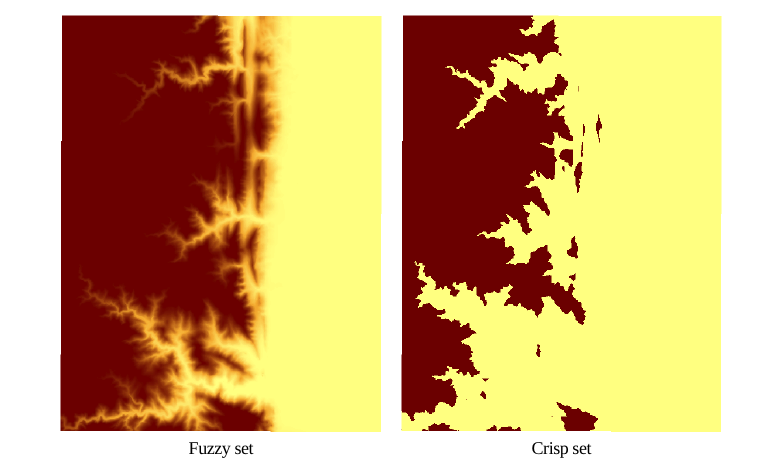
\includegraphics[width=\textwidth]{fuzzy}
      \caption[This is an illustrative example of an analysis with a fuzzy logic approach (left) and a crisp approach (right);]
{This is an illustrative example of an analysis with a fuzzy logic approach (on the left) and a crisp approach (on the right)~\cite{fuzzy3};}
      \label{fuzzy} % so that one can \ref it elsewhere	
    \end{center} 
  \end{figure}

\clearpage

\section{Key Aspects of the System}\label{key}
In this section we describe key aspects of the system, that implements the tools listed on section~\ref{objectives}. These recommendations are a result of the review on~\ref{context}, and also of the "hands-on" experience of developing fishery data management systems. Some of these aspects may be innovative in the fishery systems context, although established practices on the software development field. Other aspects may be a reaction towards negative practices that we experienced or, on the contrary, positive trends that we wish to support.\\
Often behind "failure" of software projects there is a disregarding of these practices, rather than technical incapacity. We understand by success, not only having a \textbf{good quality, working software, delivered on time, but also to have a system that will continued to be used, maintained and improved by the community}.

\subsection{AGILE Approach}\label{agile}
\emph{AGILE software development}~\cite{agile} is a group of software development practices based on iterative and incremental development; in this framework, requirements and solutions evolve through collaboration between self-organizing, cross-functional teams. There is an emphasis on software quality, adaptation to change, and involvement of team members, that is resumed in the twelve principles of the AGILE manifesto:
\begin{itemize}
\item Customer satisfaction by rapid delivery of useful software.
\item Welcome changing requirements, even late in development.
\item Working software is delivered frequently (weeks rather than months).
\item Working software is the principal measure of progress.
\item Sustainable development, able to maintain a constant pace.
\item Close, daily co-operation between business people and developers.
\item Face-to-face conversation is the best form of communication (co-location).
\item Projects are built around motivated individuals, who should be trusted.
\item Continuous attention to technical excellence and good design.
\item Simplicity- The art of maximizing the amount of work not done - is essential.
\item Self-organizing teams.
\item Regular adaptation to changing circumstances.
\end{itemize}

  \begin{figure}[!ht]%[htbp]
    \begin{center} 
	\includegraphics[width=0.5\textwidth]{Agile_Software_Development_methodology}
      \caption[Agile Software Development methodology;]
{Agile Software Development methodology;\\ source: \url{https://en.wikipedia.org/wiki/Agile_software_development}}
      \label{agile-pic} % so that one can \ref it elsewhere	
    \end{center} 
  \end{figure}

In a "traditional" approach for software development, e.g. the \emph{Waterfall} model, "change" is a threat to the completion of the project. After "closing" the requirements stage, any changes in the design of the software are counter productive, and will inevitably slow-down the whole process (or condemn it to failure). However good ideas come usually in the late stages of the traditional development cycle, when we already saw some results. For instance, we may create separated forms for introducing logbook and sampling data. However, when we are "demoing" the program we may actually find out that they are quite similar, and probably we could reuse most of the form (and the storage system as well!). We are close to the delivery date, and this change would imply refactoring the entire system, so we have to choose between delaying everything or disregarding the "new idea". With this approach, software systems often lack creativity. AGILE methodology instead makes a point of embrassing change, as something 
positive.\\
SCRUM~\cite{scrum} is an AGILE development framework, focused on project management institutions where it is difficult to plan ahead; this is often the case of cross disciplinary projects, involving many different stakeholders.\\
According to~\cite{scrum_guide}, the SCRUM team roles are: product owner (PO), SCRUM master and developing team. The PO is the person who knows everything about the product - he represents the stakeholders; he is also the person responsible for creating and maintaining the \emph{product backlog}. The backlog, can be regarded as a "wish list", or a collection of use cases with everything we want the application to do. The backlog may, and should be adjusted during the development cycle. The PO should have full authority over the management of the backlog. The backlog allows to use interesting progress tools, such as the "burn down chart" where we track the progress of the project, and are able to forecast release dates, based on the "burn down velocity".\\
A \emph{Sprint} is a short development cycle (weeks to months, depending on the project) where a series of selected items from the backlog are considered "done". The responsible for turning backlog items into incremental development during the the Sprint, belongs solely to the development team and they should have full decision power on "how" they are going to do it. In SCRUM teams there is no project manager, but the equivalent to it would be the SCRUM master. He helps everyone to change the interactions to maximize the value created by the Scrum Team. The SCRUM master interacts with the development team, PO and organization.\\
The interactions between team members are very important and they are one of the things that makes AGILE projects adaptable. On SCRUM, we have a "daily SCRUM" which is a very short meeting among the development team, to track progress and tackle possible difficulties. At the end of each Sprint there are meetings involving the entire team:  a "Sprint review" and a "Sprint retrospective"; the review is focused on the product, while the retrospective is focused on the process. During the review, the SCRUM master marks items as "done", where "done" does not mean software that "looks like it is working", with disorganized code and without testing, but it means "ready to be released", including documentation and testing. After this, the items for the next Spring are defined.\\
SCRUM \textbf{does not solve the development problems}, but it makes them visible and enables targets, with short cycles, that leave room for experiments.\\
According to~\cite{primer}, the application of SCRUM methodologies has brought noticeable improvement in: productivity, moral of the team, adaptability, responsibility, collaboration and cooperation; in places such as: Yahoo!, Microsoft, Google, Lockheed Martin, Motorola, SAP, Cisco. In the following lines, we list a set of SCRUM recommendations that could be very valuable on the context of this project:
\begin{itemize}
\item \textbf{Continuous integration and often releases}: This could be achieved by using a versioning system (e.g.: Git) and automated buildings (e.g. every night), with automated generation of documentation (e.g.: Doxygen); using these tools the software would be ready to "release" at any moment (e.g., when decided by the PO), with minimum effort.
\item \textbf{Cross-functional, self organized development teams}: Till a certain extent there could be some specialization of some members of the development team (for instance in "databases"), but is proved to be much more productive when everybody can do all work, and transfer knowledge; in this way during the Sprint, it is possible to concentrate the effort of the team in the parts where it is more necessary; it is also less "damaging" for the project, if a member of the team is absent, or if he decides to leave.
\item \textbf{Test team}: There is an exception to the previous point, which is the test team. It is desirable that the members of the development team can also be testers, but this should not replace the role of an independent tester. Professional testers, design tests that the SCRUM team would not imagine or did not have the hardware to implement. They play the role of the "users" and access the system in exactly the same way that users will. The advantage of using a tester rather than stakeholders, is to reduce the testing period by using an efficient methodology.
\item \textbf{Flexible, "bottom-up", decisions regarding adopting of software frameworks and tools}: The decisions about development should be left to the people who are going to implement it; there should be no hierarchies within the development team (there is no such thing as "lead developer"); everybody is labelled as "developer".
\item \textbf{Size of the development team}: While there are stages when it is useful to program alone, it has been observed that fewer than three development team members decreases interaction and results in smaller productivity gains~\cite{scrum}. The minimum size of development team has been set to three. Part-time members are something to avoid, as it is important to have their fully commitment during the Spring.
\item \textbf{Sustainable rhythm of work}: It has been observed that when developers are not driven to work long hours, they are more "energetic" in their work, and often more creative~\cite{xp}.
\item \textbf{Use of incremental design}: Start with a simple working system and add features improve, and refactor, instead of choosing very complicated designs in the beginning, that will "freeze" the entire system for a long time.
\item \textbf{Adaptability to change}: in order to face change, there should be flexibility in at least one of these three components: price, time or functionality.
\item \textbf{Meet often}: In the case of geographically distributed teams, it is possible to promote meetings using the internet. Skype can be used for conference calls, and forums or chats can support discussion; From time to time, it is also useful to bring the team together in one location.
\item \textbf{Involvement of the stakeholders}: A stakeholder is anyone who is a direct user, indirect user, manager of users, senior manager, operations staff member, the "gold owner" who funds the project, support (help desk) staff member, auditors, developers working on other systems that integrate or interact with the one under development, or maintenance professionals potentially affected by the development and/or deployment of a software project; it is important to engage as many stakeholders as possible in the backlog review; one way of keep them informed (and involved) is the use of a wiki page for discussion, and to present results (as an example, see~\cite{ladybug}).
\item \textbf{Frequent refactoring with emphasis on non-functional characteristics of the software}: For instance: expressiveness of the code, re-usability, etc; the use of good design patterns will ease the debugging and the development of new features, and will increase the collective ownership of the code; software that did not focused on non-functional characteristics can quickly become obsolete, defeating the purpose for which it was built in the first place.
\end{itemize}    
To summarize, the key benefits of embrassing AGILE practices are: \textbf{ability to meet deadlines, ability to face "changes", satisfaction across the community} and ultimately, \textbf{good quality software}.\\
Based on the ideas exposed above, we propose an AGILE/SCRUM project team of four people and three roles:
\begin{itemize}
\item One product owner;
\item One SCRUM master, that also doubles as developer;
\item Two multi-functional developers, that also double as testers;
\end{itemize}
Temporarily we may also need to add a "supporting cast", that helps the PO and the development team to perform specialized tasks (see figure~\ref{agile-pic}).
\begin{itemize}
\item \textbf{Technical experts}: Temporarily the team may need the help of technical experts to help them overcome a difficult problem, and to transfer their skills to one or more developers on the team (e.g.: database expert, GIS expert).
\item \textbf{Domain experts}: As the PO represents a wide range of stakeholders (not just end users), it isn't reasonable to expect him to be an expert at every single nuance of the domain. Thus the PO may sometimes bring in domain experts to work with the team (e.g.: African small-scale fisheries expert, small-scale fisheries statistical systems expert). 
\item \textbf{Independent tester}: Effective AGILE teams often have an independent tester working in parallel, that validates their work throughout the software lifecycle. 
\end{itemize}

  \begin{figure}[!ht]%[htbp]
    \begin{center} 
	\includegraphics[width=0.8\textwidth]{agileTeamSmall}
      \caption[Organization structure of a small agile team;]
{Organization structure of a small agile team; on a SCRUM team, the team lead is replaced by the SCRUM master;\\ source: \url{http://www.ambysoft.com/essays/agileRoles.html}}
      \label{agile-pic} % so that one can \ref it elsewhere	
    \end{center} 
  \end{figure}

\subsection{Alternatives to the Relational Model}\label{nosql}
The reviewed systems on section~\ref{context} have one thing in common: they use a relational database. The relational model was developed by Edgar F. Codd in 1969~\cite{relational}, as a declarative method for specifying data and queries. It is very established in the software world, it has a strong theoretical (mathematical) basis behind it, and a large number of experienced users that are able to provide a good support. However "antiquity" and "reputation" do not mean that this model is suitable and should be adopted for every situation, as it is often the case.\\
The relational model is a top-down approach, where we "know everything" about our data. While this may be true for some cases, it is probably not the case of fishery data management systems, where often requirements change over time. For instance a logbook sheet, may include a couple of fields at first, but with user experience we may decide that we want to readjust it and remove some obsolete fields, and add new ones. We may also decide to readjust it because we want to integrate a logbook from another country, that has a completely different structure. Although it is possible to "refactor" a relational database , it is always a "painful" and time consuming experience, specially if it already contains data that needs to be migrated. This is because relational databases rely on a "strong" view about "what" the data should be (the schema), that is more important than the data itself . They are not flexible and they are not AGILE (see~\ref{agile}). Once we accept that we do not "know everything" about our data,
 
than perhaps we should look for a model that complies to this fact.\\
NoSQL~\cite{nosql} is a broad class of Database Management Systems (DBMS) that do not adhere to the relational model. In the NoSQL model the ability of storing and retrieving large quantities of data is more important than the relationships between elements. These are some interesting features of NoSQL databases:
\begin{itemize}
\item They are a good fit for object-oriented programming models; for instance, they enable to represent hierarchical structures such as trees.
\item They are designed as distributed systems, which means they scale very well. Their ability to store, manipulate and analyze ever increasing volumes of data can be maintained without increasing the computational power (more processors or hard-drives); we just need to add more nodes to the system, instead. 
\item They support data replication, to ensure high-availability and support disaster recovery. This means the the "merging" of databases is directly supported by the system.
\end{itemize}
The CAP~\cite{cap} theorem, which applies to many sorts of distributed systems - such as NoSQL databases - states that it is impossible for a distributed computer system to simultaneously provide all three of the following guarantees:
\begin{itemize}
\item Consistency: All nodes see the same data at the same time.
\item Availability: 100\% of requests are completed successfully.
\item Partition Tolerance: Any given request can be completed even if a subset of nodes in the system are unavailable.
\end{itemize}
Many NoSQL systems, "sacrifice" consistency, in exchange of availability and partition tolerance. These systems are called "eventual consistent"~\cite{consistency}, which means that given a sufficiently long period of time over which no changes are sent, all updates can be expected to propagate eventually through the system and all the replicas will be consistent. NoSQL systems do not need to be "eventually consistent", but they may choose to do so.

Finally it is important to consider the cases where we wish to achieve scalability, without "sacrificing" consistency and transactions. For those situations it is perhaps pertinent to consider an hybrid solution, using a relational database to store the relations and a NoSQL to store the actual data. There are also some hybrid SQL-NoSQL solutions on the market, that combine advantages of both systems; these are called "NewSQL" databases.

\subsection{Redefining the Centre of the Application}\label{nodb}
One common mistake when designing an application is to put the database or the framework as the centre of the application; e.g.: when designing fishery management systems, it is very common to start by choosing the technology (e.g.: .NET Framework, Oracle) or to design the database before deciding anything else (including, if we have the "need" for a database). This is wrong, as the centre of the application - the highest level and most visible architectural entities - should always be the "use cases"~\cite{unclebob}. The first thing should be to know "what" exactly are the data entities involved (the "actors"), how they are related, and how they are used. Only after clarifying these points it is possible to make decisions about a data model, and fit it into a database. Getting a database "involved earlier on" will warp the design, and influence our ideas about what we want to achieve. For instance, the relational model will bias our thinking into a "relational" view of the world, where data is organized 
into 
tuples and relations~\cite{relational}.\\
Databases and frameworks are technical details that may be decided (and changed) later, but a correct design is a crucial - and often disregarded - step in software development.\\
In an AGILE approach (see section~\ref{agile}), developing use cases is regarded as an iterative process; the process should rely on work and refinement, rather than getting them at perfection in the first instance~\cite{usecases}. The primary use cases should be the "sunny day" scenarios; these are scenarios that describe what happens when everything "goes well". These scenarios are very important, firstly because they account for what happens in most of the cases, and secondly because they will help us write the edge cases, or "Rainy day" scenarios.\\

\subsection{Identifying Reuse Opportunity for Use Cases}\label{reuse}
When designing the system, and particularly when writing the "use cases", it is pertinent to identify opportunities for generalization. Object oriented languages provide a good framework for generalization through "inheritance".\\
For instance, we may have different types of landing sites, such as "Ports" or "Freezer Boats". If we create an entity "Port", later we will have to create another entity "Boat" copying some of the properties of the "Port" (e.g.: name). If we create instead an object "Abstract Landing Site", we can derive from it entities "Port" and "Boat", ihneritating common characteristics and adding specific ones (for instance the port may also have geographic coordinates, and the boat may have a license plate). Moreover we don't need to refactor any code that referred to generic properties of the "Port", when creating the "Boat" entity, and later we may decide to introduce other entities that we did not planned in the beginning, such as "Virtual Landing Sites".\\
The benefits of generalization are that in one hand we eliminate duplicate behavior and attributes, but most importantly that we make the system more understandable and flexible. The relational model does not provide a good framework for generalization as it does not "understand" the concepts of "objects" and "inheritance". For this reason, there are some "clashes" between the object oriented thinking promoted by many programming languages and the relational model implemented in many databases. It is possible to connect these two models, but always at the expenses of complex and non-intuitive solutions that often involve a lot of code. On section~\ref{nosql} we already discussed some alternatives to the relational model, that are more "friendly" for object oriented programmers.

\subsection{Use of Free and Open Source Software}\label{foss}
Free and open source software (FOSS) is software that is both \emph{free} and \emph{open-source}. Nowadays the two software movements have drifted apart, so it is important to use a full definition. According to the Free Software Foundation~\footnote{\url{http://www.fsf.org/}}(FSF), a "free" software must be licensed to guarantee four types of freedom: \emph{freedom to use, study, share and modify that software}. In this definition "free" is not synnonim of "zero cost", although it may be distributed with no charges. An open source license makes source code available to the general public with relaxed or non-existent copyright restrictions.\\
Apart from ethical reasons which are mainly connected to the "free software movement" (see~\cite{free}), there are many motivations to switch to a free and open-source model. Namely:% Usually the most popular argument is the zero cost. This is important, but there is a lot of software that does not charge any fee but does not benefit from other advantages of this model (e.g.: ESRI ArcExplorer, Internet Explorer, Skype).
\begin{itemize}
\item \textbf{Lower software costs}: Normally FOSS is free and may charge only for support or documentation. If we develop strictly using tools and libraries that follow this model, developing countries will not have to fight with budget restrictions to use, maintain and develop the software. In this way we increase the possibility of ownership by recipient countries.
\item \textbf{Lower hardware costs}: Generally, FOSS is compact and portable, and as a result it requires less hardware power to accomplish the same tasks as on conventional servers (Windows, Solaris) or workstations. Thus it is still possible to use less expensive or older hardware, allowing to install it in  countries with less resources.
\item \textbf{Simplified license management}: You may obtain as many licenses as you want, to install everywhere, which means that productivity will not be affected by licensing issues.
\item \textbf{Wide support}: Support for FOSS is often superior to proprietary solutions. This is because we have two levels of support: the free one, that is available through the online community and the paid one, that many tech companies now provide (e.g.: Novell).
\item \textbf{Software quality}: The peer review process and community standards, plus the fact that source code is disclosed to everyone, tend to drive excellence in design and efficiency in coding.
\item \textbf{Extended lifetime}: The availability of the source code and the right to modify it enables the unlimited improvement of the software. It also enables to port it to a new hardware or operative system. In reality, no binary-only applications survived more than 10 years in an unmodified form, while many open software systems have survived more than 30 years.
\item \textbf{Frequent updates}: You do not need to be a programmer to benefit from the availability of the source code; these freedom attracts a community of developers that fixes bugs and develops new features; the right to distribute the modified versions allows the community of users to benefit from all these improvements.
\item \textbf{Growing community}: The right to use the software in any way, combined with redistribution rights, may attract a large population of users, which helps in turn to build up a market for support and customization of the software, which will attract even more developers to work in the project. If the software is useful, there is a feedback which will drive the quality of the product, improve its functionality and its support.
\end{itemize}
There are many problems linked to the use of traditional software, that can be solved using FOSS. 
\begin{itemize}
\item \textbf{No one can restrict in a unilateral way how the software is used (even older versions)}: Sometimes a proprietary software vendor decides to discontinue a software product for an older platform (e.g. Windows 95); in this case the users can either stick to the old version not benefiting from new updates, or switch to another product. In an FOS model, the costumers can keep developing for the desired platform, or alternatively fund somebody to do it. %It is also possible that a third party already took that task.
\item \textbf{The future of the software is not dependent on a single entity}: With the recent merges in the proprietary software market that led to the "cannibalization" of some software, it is not uncommon that a company decides to completely discontinue a product. In this case, no one is able to prevent the "killing" of the software. In a FOS model, if a company decides to stop development it is always possible to find another alternative, even if it means funding another group to do it.
\item \textbf{There are no "black boxes"}: By having the source code available, it is possible to assess the correctness of the algorithms and of the implementation scheme used. In the case of scientific applications this may be a very important point, since the quality of the results depends on the correctness of the algorithms. FOSS also grants people the freedom to modify (and share) the code, and therefore they may correct or improve an algorithm, if there is such need.
\item \textbf{It provides a new forum for democratic action}: As individuals, not companies, decide the overall direction of progress and there are no market forces behind it, there is a more democratic model that allows people with opinions (even if they do not have financial resources) to participate in the improvements of the system.
\end{itemize}
There are also some arguments against FOSS, some of which are "myths", or are no longer true.
\begin{itemize}
\item \textbf{There is no support available}: some companies/organizations demand a support model, similar to the one provided by proprietary software. This support is currently available at the same fees, or lower of proprietary software support (e.g. Novell).
\item \textbf{Development resources are scarce}: Linux and open source are actually the largest segment of the developers universe. Most of the developers tools, languages and processes have a free and open source port. For instance the .NET frame has been implemented with Mono~\footnote{http://www.mono-project.com/Main\_Page}.
\item \textbf{There is no training available}: this used to be true, but not anymore. Many companies nowadays provide training and multiple levels of certification in Free and Open Source technologies~\footnote{for instance, Faunalia - ~\url{http://www.faunalia.pt/}}.
\item \textbf{All open source is a work-in-progress}: this may be true for some software but not all. Although FOSS is evolving constantly, we already see some stable, secure and quality solutions (e.g. Apache, PostgreSQL, QGIS). Although some projects are still maturing, many others are already "usable" as they are.
\item \textbf{It is difficult to use}: this also used to be true, but not anymore. Initially, FOSS required some advanced knowledge of operative systems (and sometimes programming), in order to be used. Nowadays, products like Ubuntu or QGIS are ready to be installed and used almost by everyone. This is both because they reached some maturity that has driven them to be stable and less "buggy", and a larger community pushed for products to become more "user friendly". %Although this is definetly a trend, it may still be argued that many FOSS products require an higher IT knowledge than their equivalent proprietary versions. However the initial investment (in time and effort) is largely compensated by all the benefits previously mentioned.
\end{itemize}
It is true that the users of FOSS are driven to be more "autonomous", since the development model is focused on individuals and communities. It is not true that FOSS is "for developers only", since as we already pointed out, everyone can benefit from involving a large community of developers.\\
Moreover since they have a wider technology choice, FOSS developers are more exposed to different frameworks/libraries and will be \textbf{more likely to try new things}, than their proprietary counterparts. That fact alone does not make them "better" programmers, but makes them at least more adaptable. Technology choices should be ultimately \textbf{driven by the nature of the problem, and not by financial/market constraints or by deficiencies of the developers}.\\
On the context of fishery data management systems, there are a lot of FOS libraries, databases, frameworks and GIS resources that can support the development of the system, in all fronts. On section~\ref{context} we verified that many systems have chosen this approach, and CAS Medfisis~\cite{medfisis} is an example of a fishery data management system that was built \emph{almost entirely} on FOS tools. On the next few paragraphs, we list examples of FOSS that covers different areas involved in the implementation of the proposed system. 
\begin{itemize}
\item Databases: MongoDB, SQLite, Postgres.
\item Spatial Extensions for Databases: SpatiaLite, PostGIS.
\item GIS: QGIS, GRASS, SpatiaLite GIS.
\item Statistics: R.
\item Developing Frameworks: Qt.
\item Support Libraries: Boost, STL, PyQGIS, GDAL.
\item Versioning System: Git.
\item Wikipedia Server: Mediawiki
\item Mockups: Pencil
\item UML: Dia
\item Documentation: Doxygen
\item GeoWebservers: Mapserver, Geoserver, Mapnik.
\item Geoweb client: OpenLayers
\end{itemize}
Note that the all software mentioned above are mature tools, that have been effectively adopted by many projects.

%link to other platforms


%\section{Project Outputs}\label{outputs}
%Write something here

%\section{Work Plan}\label{plan}
%Write something here

%\section{Capacity Building Components}\label{capacity}
%Write something here

%\section{FAO Input}\label{fao}
%Write something here

%\section{Recipient Countries Input}\label{countries}
%Write something here

%\section{Project Budget}\label{budget}
%Write something here

%AKNOWELEDGMENTS

%\section{Project Outputs}\label{outputs}
%Write something here

\section{Aknoweledgments}
I would like to thank Henrik Degel, from the Fishframe project, for kindly providing me with a login that allowed me to try the Fishframe system; Carlos Pinto, from ICES, for amending and "filling the gaps" for the ICES systems reviewed on section~\ref{context}; and Fabio Carocci, from FAO, for suggesting me to review a proprietary GIS fishery system. Finally, I would like to thank the agile-spain-barcelona google group, for removing some of my doubts about AGILE/SCRUM, and for pointing me to valuable reference items on this area.
\clearpage

\begin{thebibliography}{9}
\bibitem{fishframe}F.\ Degel, T.\ Jansen {\em FishFrame Fisheries and stock assessment data framework}. ICES CM 2006/M:02
, 2006.
\bibitem{fishframe1}F.\ Degel, T.\ Jansen {\em FishFrame Licensing}.Danish Institute for Fisheries Research
Charlottenlund castle, Charlottenlund, Denmark. 5th March, 2006.
\bibitem{intercatch}H.\ Kjems-Nielsen, L. \ Inger Larsen, M.\ Zarecki1, T.\ Jansen, B.\ Cowan, P.\
Sandbeck, M.\ Dueholm, O.\ Skov.{\em InterCatch - a tool for fish stock assessment, status and methods}. ICES CM 2006/M:29, 2006.
\bibitem{intercatch1}ICES. {\em InterCatch - User Manual.}. Document version 1.9.
\bibitem{EcoSystemData}ICES {\em EcoSystemData3.0\_Release}. \url{http://ecosystemdata.ices.dk/EcoSystemData3.0_Release.pdf}
\bibitem{tuna}M.\ Stocker, H.\ Stiff, W.\ Shaw, A.W.\ Argue {\em The Canadian Albacore Tuna Catch and
Effort Relational Database}. Canadian Technical Report of Fisheries and Aquatic Sciences 2701, 2007.
\bibitem{mappamond}Mappamond {\em Fishery\_Analyst\_V2\_manual}. \url{http://www.mappamondogis.it/pdf/Fishery_Analyst_V2_manual.pdf}
\bibitem{victoria}L.I.\ Muhoozi {\em Implementation of a Fisheries Management Plan
(IFMP) Project for Lake Victoria: A Report Of The Fisheries Catch Assessment Survey
In The Ugandan Waters Of Lake Victoria For The February 2008 Survey}. National Fisheries Resources Research
Institute (NaFIRRI) and National Agricultural Research
Organization (NARO), February, 2008.
\bibitem{dominican}P. A.\ Medley {\em Review Of The Data Collection And Management
Systems Of The Marine Fisheries In The Dominican
Republican: Final Report}.
\bibitem{samoa}N.\ Helm {\em A Report on The Market Survey of Reef and Lagoon Fish Catches In Western
Samoa}. South Pacific Comission, SPC/lnshoreFish.Res./BP 30, 7 March 1988.
\bibitem{medfisis} FAO.\emph{Medfisis},\url{http://www.faomedfisis.org/}.
\bibitem{json} JSON.\emph{JSON},\url{http://json.org/}.
\bibitem{sqlite} SQLite.\emph{SQlite},\url{http://www.sqlite.org/}.
\bibitem{fuzzy}H.H.\ Shahri, A.A.Z.\ Barforush.{\em Data mining for removing fuzzy duplicates using fuzzy inference}.
Fuzzy Information, 2004. Processing NAFIPS '04. IEEE Annual Meeting, 27-30 June 2004. \url{http://ieeexplore.ieee.org/xpl/freeabs_all.jsp?arnumber=1336319}
\bibitem{outliers}C.\ López.{\em Quality of Geographic Data
Detection of Outliers and Imputation of
Missing Values}. PhD Dissertation on the Royal Institute of Technology, Department of Geodesy and Photogrammetry, Stockholm, Sweden 1997.
\bibitem{ices}ICES.{\em Workshop on methods for merging metiers for
fishery based sampling (WKMERGE)
}. ICES WKMERGE REPORT 2010, Copenhagen, Denmark, 19-22 January 2010.
\bibitem{morocco}R.\ Forrest, T.\ Pitcher,
R.\ Watson, H.\ Valtýsson,
S.\ Guénette {\em Estimating Illegal and Unreported Catches from Marine Ecosystems: Two Case Studies}. Sea Around Us: North Atlantic, Page 81, 19 DEC 2002.
\bibitem{ices2} ICES.\emph{ICES Data Centre},\url{http://www.ices.dk/datacentre/Submissions/index.aspx}.
\bibitem{geocrust}J.\ Simoes, C.\ Pinto, M.\ Afonso-Dias. {\em Methodology for Monitoring and  Management of the Crustacean Trawl Fleet. Example of GeoCrust 1.0 GIS} in Finisterra special edition Cartography and Geographic Information Systems, 2005.
\bibitem{fuzzy2}D. Z.\ Sui {\em A Fuzzy Gis Modeling Approach Land Evaluation For Urban}. Environ. and Urban Systems, Vol. 16, pp. IOl-115, USA, 1992.
\bibitem{fuzzy3}W.\ Kainz.{\em The mathematics of GIS}. \url{http://goo.gl/fb/CWklR}
\bibitem{fao1}FAO/DANIDA.{\em Guidelines for the Routine Collection of Capture Fishery Data}. FAO FISHERIES TECHNICAL PAPER 382. Food and Agriculture Organization of the United Nations. Rome, 1999.
\bibitem{bd}{\em fisheries\_data\_mng\_sys.sqlite}.
\bibitem{first}L. R.\ Garces, G. T.\ Silvestre, I.\ Stobutzki, F. C.\ Gayanilo Jr, F.\ Valdez, M.\ Saupi, T.\ Boonvanich, M.\ Roongratri, P.\ Thouc, Purwanto, I.\ Haroon, K. N.\ Kurup, M.\ Srinath, H. A. B.\ Rodrigo, M. D.\ Santos, F. S. B. Torres Jr., M. K.\ Tan, D.\ Pauly {\em A regional database management system—the fisheries resource information system and tools (FiRST): Its design, utility and future directions}. Fisheries Research, 78 (1-2). pp. 119-129.
\bibitem{pescart}IIP.{\em PESCART: Documentacao tecnica}. 2006.
\bibitem{cost}European Comission.{\em Common tool for raising and estimating properties of statistical estimates derived from the Data Collection Regulation (COST)}. Studies and Pilot projects for carrying out the common fisheries policy. Call for proposal FISH/2006/15 – lot 2.
\bibitem{cost1}COST Team and various contributors.{\em Package ‘COSTcore’ documentation}. February, 15, 2008.
\bibitem{kongatora}B. U.\ Ibrahim, J.\ Auta, J. K.\ Balogun,{\em A Survey Of The Artisanal Fisheries Of Kontagora Reservoir, Niger State, Nigeria}. Bayero Journal of Pure and Applied Sciences, 2(1): 47 - 51. 2009.
\bibitem{unclebob}Uncle Bob. \emph{NO DB}. \url{http://blog.8thlight.com/uncle-bob/2012/05/15/NODB.html}
\bibitem{usecases}Gatherspace. \emph{Writing Effective Use Case Examples}. \url{http://www.gatherspace.com/static/use_case_example.html}
\bibitem{relational}Wikipedia. \emph{Relational model} \url{https://en.wikipedia.org/wiki/Relational_model}
\bibitem{nosql}Wikipedia. \emph{NoSQL} \url{https://en.wikipedia.org/wiki/NoSQL}
\bibitem{consistency}Wikipedia. \emph{Eventual Consistency} \url{http://en.wikipedia.org/wiki/Eventual_consistency}
\bibitem{cap}Wikipedia. \emph{CAP} \url{https://en.wikipedia.org/wiki/CAP_theorem}
\bibitem{agile}AGILE. \emph{Manifesto} \url{http://www.agilemanifesto.org/}
\bibitem{ladybug}GISFOREAF. \emph{Project Wiki Page} \url{http://ladybug.no-ip.org:8010/mediawiki/index.php/GISforEAF}
\bibitem{ambysoft}Ambysoft. \emph{Roles on Agile Teams: From Small to Large Teams} \url{http://www.ambysoft.com/essays/agileRoles.html}
\bibitem{scrum}Wikipedia. \emph{SCRUM} \url{http://en.wikipedia.org/wiki/Scrum_(development)}
\bibitem{scrum_guide}K.\ Schwaber, J. Sutherland{\em The Scrum Guide. The Definitive Guide to Scrum: The Rules of the Game}. 1991-2011.
\bibitem{primer}P.\ Deemer, G.\ Benefield, C.\ Larman, B.\ Vodde {\em INFORMACIÓN BÁSICA DE SCRUM (THE SCRUM PRIMER)}. Version 1.1. SCRUM Training Institute.
\bibitem{xp}H.\ Kniberg{\em SCRUM Y XP DESDE LAS TRINCHERAS Cómo hacemos Scrum}. Version 1.1. Enterprise Software Development Series.
\bibitem{free}S.\ Williams{\em Free as in Freedom}. 2002. Project Gutenberg.
\end{thebibliography}
\end{document}
